\documentclass[11pt]{article}

\usepackage[review]{acl}
\usepackage{times}
\usepackage{latexsym}
\usepackage[T1]{fontenc}
\usepackage[utf8]{inputenc}
\usepackage{microtype}
\usepackage{inconsolata}
\usepackage{amsmath,amssymb,amsthm}
\usepackage{graphicx}
\usepackage{booktabs}
\usepackage{enumitem}
\usepackage{url}

\IfFileExists{references.bib}{}{%
  \PackageError{SRP}{Missing references.bib}{Place references.bib in first_paper/latex/ before compiling.}%
}
\IfFileExists{../../srp_experiment/results/paper_figure_pack/main_3panel_figure.png}{}{%
  \PackageError{SRP}{Missing main 3-panel figure}{Place the image under srp_experiment/results/paper_figure_pack/ or update the path in main_submission.tex.}%
}
\IfFileExists{../../srp_experiment/results/paper_table.tex}{}{%
  \PackageError{SRP}{Missing paper table}{Generate srp_experiment/results/paper_table.tex before compiling.}%
}
\IfFileExists{../../srp_experiment/results/quality_table.tex}{}{%
  \PackageError{SRP}{Missing quality table}{Generate srp_experiment/results/quality_table.tex before compiling.}%
}
\IfFileExists{../../srp_experiment/results/efficiency_table.tex}{}{%
  \PackageError{SRP}{Missing efficiency table}{Generate srp_experiment/results/efficiency_table.tex before compiling.}%
}
\IfFileExists{../../srp_experiment/results/guardrail_table.tex}{}{%
  \PackageError{SRP}{Missing guardrail table}{Generate srp_experiment/results/guardrail_table.tex before compiling.}%
}
\IfFileExists{../../srp_experiment/results/camera_ready_table.tex}{}{%
  \PackageError{SRP}{Missing camera-ready table}{Generate srp_experiment/results/camera_ready_table.tex before compiling.}%
}

\title{Semantic Runtime Protocol: Core Submission Version}
\author{Anonymous Author(s)\\Affiliation\\Address\\\texttt{email@domain.com}}

\begin{document}
\maketitle

\begin{abstract}
Long-horizon LLM systems often preserve context through prompt accumulation, summarization, or retrieval, but these strategies do not explicitly model semantic state as a runtime object. We present \textbf{Semantic Runtime Protocol (SRP)}, a minimal runtime abstraction for studying bounded semantic drift under repeated compression-recovery cycles. The paper asks one narrow question: whether explicit semantic-state management can improve finite-horizon stability while remaining token-efficient. We evaluate SRP against lightweight baselines under a reproducible qualification-gated experiment pipeline. The resulting claim is intentionally modest: SRP is a bounded runtime abstraction for semantic stability, not a semantic operating system.
\end{abstract}

\section{Introduction}
The central limitation in long-horizon LLM interaction is the lack of a formal runtime abstraction for semantic state. Existing prompt, memory, and retrieval systems manage tokens or stored context, but they do not make semantic transformation, validation, recovery, and update first-class runtime operations.

We study SRP as a semantic-state runtime abstraction with four operators:
\begin{itemize}[leftmargin=*]
  \item compression
  \item recovery
  \item validation
  \item update
\end{itemize}

The first paper is intentionally narrow: it tests whether explicit semantic-state management improves finite-horizon stability under repeated transformation, relative to lightweight baselines.

\subsection*{Contributions}
\begin{enumerate}[leftmargin=*]
  \item SRP as a minimal semantic-state runtime abstraction.
  \item Bounded semantic drift as the primary stability lens.
  \item A reproducible qualification-gated evaluation pipeline.
\end{enumerate}

\subsection*{Failure Boundary}
SRP is not guaranteed to work if the semantic vocabulary is corrupted, validation is unreliable, recovery becomes non-invertible in practice, or cumulative drift exceeds the tolerance budget. The paper treats this boundary as part of the claim.

\section{Related Work}
SRP is positioned against four groups of prior work:
\begin{itemize}[leftmargin=*]
  \item prompt compression and context reduction
  \item memory-augmented and retrieval-based systems
  \item agent frameworks and trajectory-based pipelines
  \item reproducibility-oriented evaluation infrastructure
\end{itemize}

The key difference is that SRP treats semantic state as an explicit runtime object rather than as token history or retrieved text alone.

\section{Runtime State and Formalization}
We model semantic state at step $t$ as:
\begin{equation}
S_t = (M_t, V_t, P_t)
\end{equation}

where $M_t$ is structured semantic memory, $V_t$ is vocabulary state, and $P_t$ is policy state. SRP defines four operators:
\begin{align}
C &: S_t \to Z_t \\
R &: Z_t \to S_t' \\
\mathrm{Val} &: (S_t, S_t') \to [0,1] \\
U &: (S_t', F_t) \to S_{t+1}
\end{align}

The formalization remains lightweight. We define observable behavior $O(S)$ and use task-relevant distance $d(O(S), O(S'))$ as semantic error. Cumulative semantic drift over repeated cycles is the main stability quantity:
\begin{equation}
\Delta_k = d(O(S_0), O(S_k))
\end{equation}

The paper uses bounded semantic drift as a practical notion for finite-horizon evaluation.

\section{Experimental Setup}
The evaluation uses one fixed workflow and a small set of methods:
\begin{itemize}[leftmargin=*]
  \item raw prompt
  \item summarization
  \item retrieval-based memory
  \item SRP
\end{itemize}

The main tasks are:
\begin{itemize}[leftmargin=*]
  \item multi-turn instruction consistency
  \item iterative compression-recovery cycles
\end{itemize}

The main metrics are:
\begin{itemize}[leftmargin=*]
  \item semantic drift
  \item task success
  \item token cost
\end{itemize}

The evaluation is qualification-gated and replayable. The experiment package includes:
\begin{itemize}[leftmargin=*]
  \item EQ gate
  \item runtime equivalence traces
  \item formal batch runs
  \item paper-ready tables
  \item paper-ready figures
\end{itemize}

\section{Results}
The main empirical claim is compact:

\begin{quote}
SRP achieves the lowest semantic drift across cycle depths and occupies a favorable low-drift, low-token regime under the qualified formal batch.
\end{quote}

The results are summarized with three linked views:
\begin{itemize}[leftmargin=*]
  \item a drift-over-cycles figure
  \item a token-cost-versus-drift Pareto frontier
  \item a contract-stability figure
\end{itemize}

Together, they show that SRP is not merely token-light or one-step stable; it preserves semantic behavior more consistently across repeated transformation while remaining competitive on efficiency.

The reader should interpret the evidence in a restrained way: SRP improves long-horizon semantic stability without claiming universal superiority or broad system replacement.

\begin{table}[t]
\centering
\setlength{\tabcolsep}{2pt}
\scriptsize
\begin{tabular}{llrlrrrrrrrrrrrr}
\toprule
B & M & C & Base & Base D & Base S & Base T & Base L & SRP D & SRP S & SRP T & SRP L & $\Delta$D & $\Delta$S & $\Delta$T & $\Delta$L \\
\midrule
\bottomrule
\end{tabular}
\caption{Comparison between Semantic Runtime Protocol (SRP) and the strongest non-SRP baseline for each backend, model, and cycle setting. The baseline is selected by task success, then semantic drift, then token cost. $\Delta$ denotes SRP minus the selected baseline. Lower drift, token cost, and latency are better, while higher task success is better. Bold indicates the stronger value within each SRP-baseline pair.}
\label{tab:srp-camera-ready-table}
\end{table}


\begin{figure}[t]
  \centering
  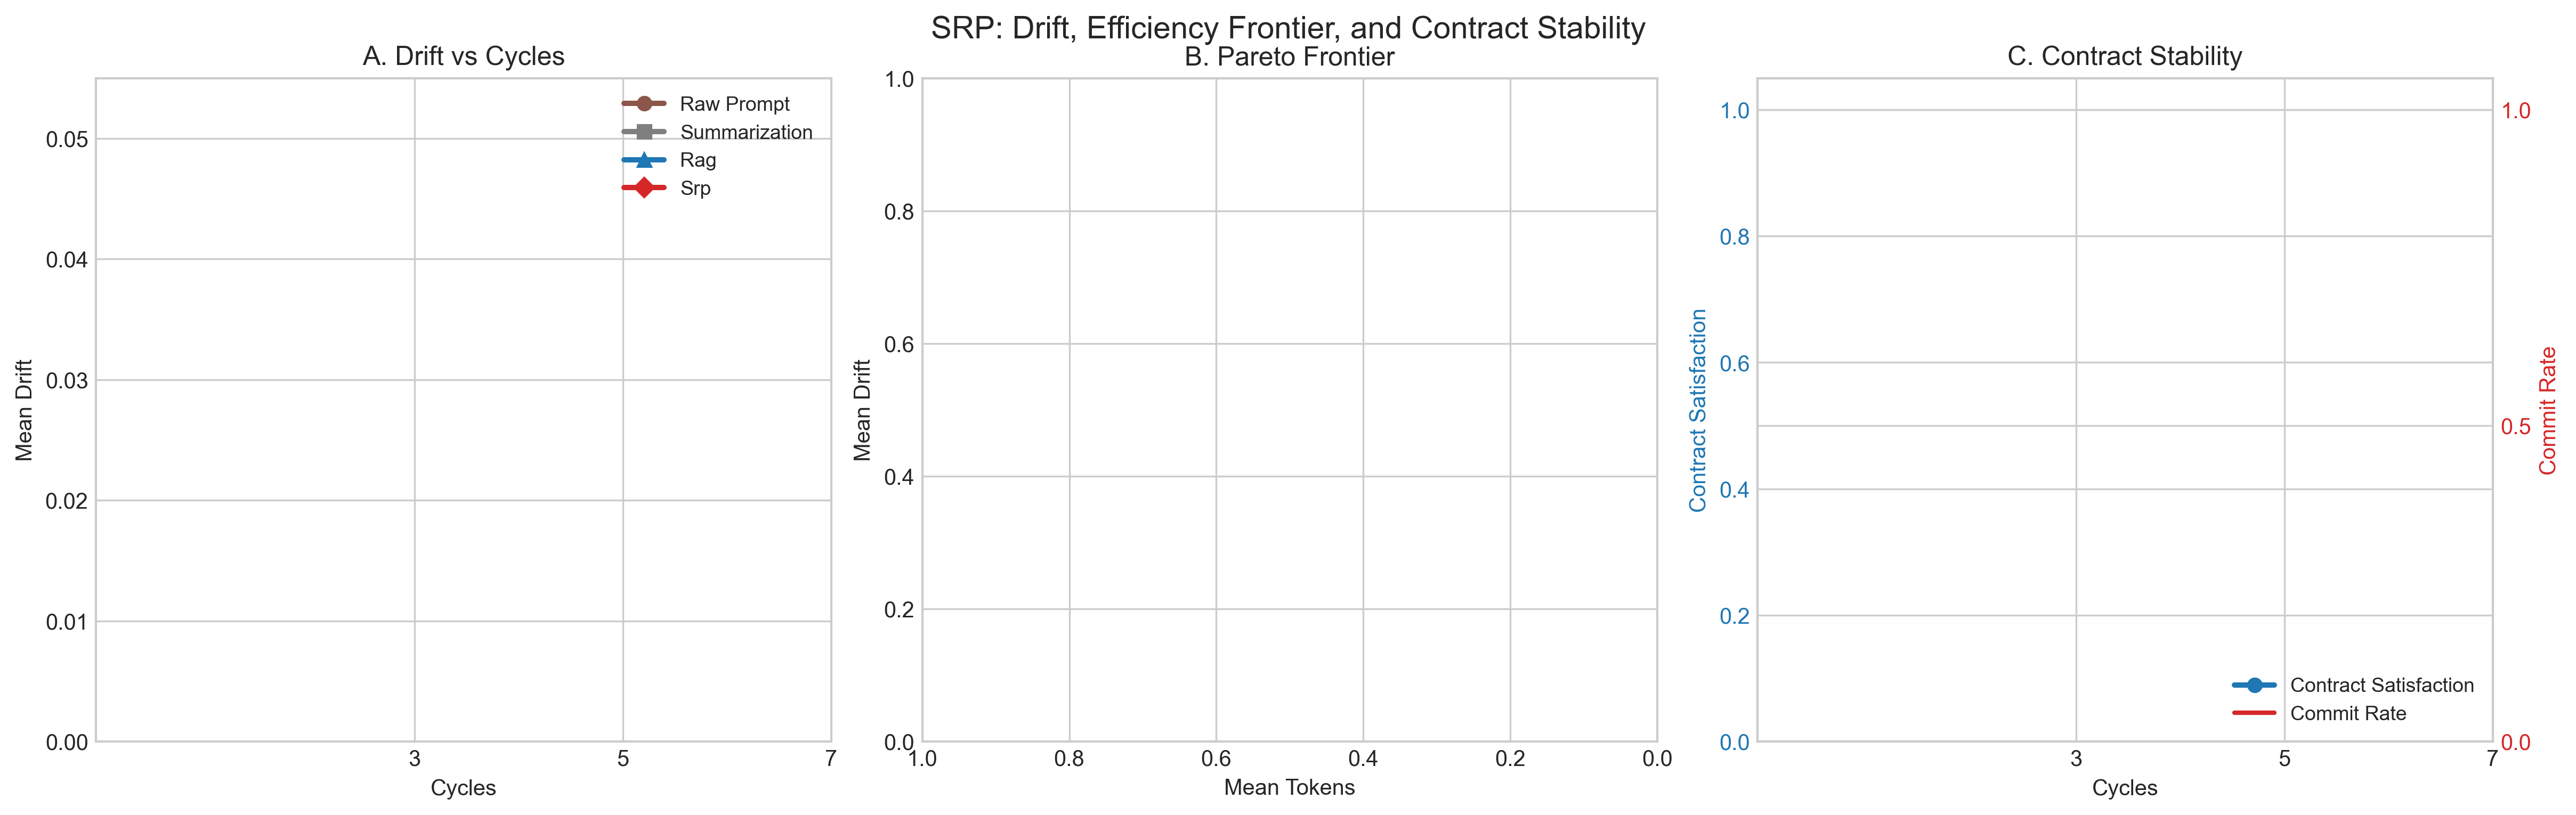
\includegraphics[width=\linewidth]{../../srp_experiment/results/paper_figure_pack/main_3panel_figure.png}
  \caption{Three-panel main results. (A) Semantic drift across cycle depths for four methods. SRP consistently achieves the lowest drift and remains stable as cycle depth increases, while summarization degrades sharply and both raw prompt and RAG exhibit substantially higher drift. (B) Token cost versus drift Pareto frontier. SRP occupies a low-drift, low-token region, indicating that improvements are not attributable to increased computational budget. (C) SRP contract stability. Contract satisfaction remains stable across cycles, and commit decisions track semantic contract compliance rather than lexical similarity, suggesting that execution stability is governed by semantic consistency rather than surface-form preservation.}
  \label{fig:main_results}
\end{figure}

\section{Discussion}
The results support a narrow reading of SRP. The paper is about finite-horizon semantic stability, not a full semantic operating system. The main discussion points are:
\begin{itemize}[leftmargin=*]
  \item why semantic state differs from memory
  \item why bounded drift is more realistic than exact preservation
  \item why the first implementation remains minimal
  \item what would be required to scale the design further
\end{itemize}

\section{Limitations}
The paper is intentionally narrow:
\begin{itemize}[leftmargin=*]
  \item finite-horizon evaluation
  \item proxy-based semantic metrics
  \item simplified state representation
  \item limited model and task scope
\end{itemize}

These constraints are part of the design, not accidental omissions.

\section{Open Questions}
The first paper preserves, rather than resolves, several questions:
\begin{itemize}[leftmargin=*]
  \item Is SRP primarily a runtime abstraction, a protocol, or a semantic communication layer?
  \item What is the minimal semantic-state object?
  \item Which drift metric should be considered the main one in the first paper?
  \item What failure cases should be shown explicitly?
\end{itemize}

\section{Future Work}
Future work can extend the present claim with:
\begin{itemize}[leftmargin=*]
  \item richer state schemas
  \item stronger validator design
  \item cross-model generalization
  \item semantic contract refinement
  \item benchmark expansion
  \item runtime lifecycle extensions such as freeze, merge, and delete
  \item transaction-style commit / rollback semantics
\end{itemize}

These are next-step extensions, not requirements for the first paper.

\section{Submission Strategy}
The most plausible near-term venues are workshop papers, short papers, student research tracks, or a technical report plus advisor feedback. The goal is a reproducible, bounded-scope paper with one strong figure and one careful framing, not a maximal full-scale systems paper.

\section{Evidence Pack}
This submission version is backed by the following qualified artifacts:
\begin{itemize}[leftmargin=*]
  \item EQ report
  \item runtime equivalence traces
  \item formal batch results
  \item drift plot
  \item contract/commit plot
  \item 3-panel main figure
  \item quality / efficiency / guardrail / camera-ready tables
\end{itemize}

If the paper is compressed further, the corresponding evidence should remain accessible through the project overview and paper-sections index rather than being deleted.

\nocite{*}
\bibliography{references}

\end{document}
